\chapter{Badania wstępne}

Projektowanie interfejsu nie może opierać się tylko na założeniach projektanta. Zgodnie z podejściem projektowym przedstawionym przez Tidwell proces ten powinien rozpocząć się od zrozumienia odbiorców \cite{Projektowanie-UI}.

Należy poznać cele, w jakich użytkownik korzysta z technologii VR, oraz elementy, które go najbardziej frustrowały podczas użytkowania. Istotne jest również ustalenie poziomu jego obycia ze sprzętem, czyli czy jest doświadczonym użytkownikiem, czy dopiero po raz pierwszy korzysta z rzeczywistości wirtualnej. Dopiero posiadając takie informacje można podejmować świadome decyzje projektowe w VR. Aby pozyskać tę wiedzę bezpośrednio od graczy VR, zdecydowano się na przeprowadzenie ankiety. 

\section{Metodologia badań wstępnych}

\subsection{Cel i znaczenie badań}

Celem przeprowadzenia ankiety było zebranie opinii użytkowników posiadających doświadczenie w korzystaniu z technologii wirtualnej rzeczywistości oraz ocena ich subiektywnych doświadczeń związanych z grami VR. Dobór respondentów z co najmniej podstawowym doświadczeniem w VR wynikał z założenia, że nawet jednorazowy kontakt z technologią pozwala użytkownikowi zidentyfikować elementy powodujące dyskomfort, frustrację lub prowadzące do rezygnacji z dalszego korzystania z aplikacji VR. Badanie zostało zaplanowane jako etap wstępny, realizowany przed rozpoczęciem projektowania i implementacji własnego rozwiązania, lecz po przeprowadzeniu analizy istniejących gier dostępnych na rynku. Jego zadaniem było potwierdzenie problemów zaobserwowanych podczas tej analizy oraz sprawdzenie, w jakim stopniu pokrywają się one z rzeczywistymi doświadczeniami użytkowników. W pracy pojęcie punktów bólu odnosi się do problemów, frustracji oraz niedogodności, na jakie użytkownicy napotykają podczas interakcji z grami VR, w szczególności w obszarze interfejsu użytkownika oraz mechanizmów interakcji. Ankieta miała na celu zarówno potwierdzenie wcześniej zidentyfikowanych punktów bólu, jak i umożliwienie ujawnienia dodatkowych problemów, które mogły nie zostać dostrzeżone na etapie analizy wybranych tytułów.

Zebrane dane stanowią podstawę do dalszych decyzji projektowych i posłużą do sformułowania założeń dotyczących projektowania interfejsu oraz interakcji w prototypie gry VR, ze szczególnym uwzględnieniem elementów wpływających na komfort użytkowania i poziom immersji.

\subsection{Pytania badawcze}

Na potrzeby badań wstępnych sformułowano pytania badawcze odnoszące się do obszarów, które w praktyce najczęściej wpływają na komfort korzystania z gier VR oraz na utrzymanie immersji. Pytania te mają charakter eksploracyjny i mogą ulec doprecyzowaniu po analizie wyników ankiety.

Sformułowane pytania badawcze:

\begin{enumerate}
    \item Jakie elementy interfejsu użytkownika w grach VR są postrzegane jako najbardziej zakłócające poczucie immersji i obecności?
    \item Jak intuicyjność, precyzja, sposób interakcji oraz układ interfejsu wpływają na doświadczenie użytkownika w VR?
     \item Jakie elementy interfejsu VR powodują dyskomfort fizyczny lub percepcyjny u użytkowników?
     \item Jak brak lub opóźnienie informacji zwrotnej w interfejsie VR wpływa na immersję i komfort użytkownika?

\end{enumerate}

Pytania ankietowe zostały opracowane w oparciu o sformułowane pytania badawcze. Szczegółowy opis struktury ankiety, podziału na sekcje tematyczne oraz rodzaju zastosowanych pytań przedstawiono w podrozdziale 4.4.

Spośród sformułowanych pytań badawczych kluczowe znaczenie miało pytanie dotyczące elementów interfejsu użytkownika, które zakłócają poczucie immersji i obecności. Stanowi ono bezpośrednie uzasadnienie podjęcia tematu pracy i punkt wyjścia do dalszych analiz projektowych. Pozostałe pytania pełnią funkcję uzupełniającą i pozwalają lepiej zrozumieć charakter zidentyfikowanych problemów, tak aby projektowany interfejs mógł zostać możliwie najlepiej dopasowany do specyfiki analizowanego typu gry VR.

Należy podkreślić, że pytania badawcze zostały sformułowane jako pytania eksploracyjne, których celem jest identyfikacja powtarzających się problemów oraz zebranie informacji wspierających proces podejmowania decyzji projektowych na etapie tworzenia prototypu.

\subsection{Metodyka badań}

W ramach badań wstępnych zastosowano podejście łączące analizę heurystyczną i badanie ankietowe.

Analiza wybranych gier VR, przeprowadzona z wykorzystaniem heurystyk użyteczności dla rzeczywistości wirtualnej opracowanych przez \textit{Nielsen Norman Group} była oparta na obserwacji i pozwoliła na wstępną identyfikacje potencjalnych problemów w projektowaniu interfejsów. Nie umożliwiała jednak jednoznacznej weryfikacji, które z tych zagadnień rzeczywiście wpływają na subiektywne doświadczenie użytkownika.

Z tego względu uzupełniono ją badaniem ankietowym skierowanym do osób już posiadających choć niewielkie doświadczenie w korzystaniu z technologii VR. Zastosowanie ankiety pozwoliło na zebranie opinii użytkowników oraz potwierdzenie istotności wcześniej zidentyfikowanych problemów z perspektywy ich rzeczywistych doświadczeń. Takie połączenie metod umożliwiło zestawienie obserwacji projektowych z opiniami użytkowników i stanowiło podstawę do dalszych decyzji projektowych. Badanie miało charakter mieszany i łączyło elementy jakościowe oraz ilościowe. Część jakościowa opierała się na analizie odpowiedzi otwartych oraz interpretacji deklarowanych doświadczeń użytkowników, natomiast część ilościowa obejmowała analizę odpowiedzi udzielanych w skali ocen. Celem badania nie było statystyczne testowanie hipotez, lecz eksploracyjna identyfikacja powtarzających się problemów oraz obszarów istotnych z punktu widzenia dalszych decyzji projektowych.

\subsection{Konstrukcja ankiety, grupa badawcza i sposób dystrybucji}

Ankieta została zaprojektowana jako autorskie narzędzie badawcze, którego konstrukcja wynikała bezpośrednio z wcześniej sformułowanych pytań badawczych. W celu ułatwienia respondentom koncentracji pytania zostały pogrupowane w sekcje tematyczne. Zgodnie z zaleceniami przedstawionymi w literaturze, długość materiału dobrano tak, aby jego uzupełnienie nie zajmowało więcej niż piętnaście minut, a pytania były podzielone na sekcje tematyczne. Miało to ograniczyć ryzyko znużenia respondentów i wynikającego z niego udzielania przypadkowych lub nieprawdziwych odpowiedzi wyłącznie w celu szybszego zakończenia badania. Uwzględniono również zróżnicowany poziom zaawansowania technologicznego ankietowanych, przez co część pytań mogła być odbierana jako bardziej lub mniej skomplikowana \cite{Ankieta,Ankieta2,Ankieta3}. 

Pierwsza część ankiety miała charakter wprowadzający i dotyczyła ogólnego doświadczenia respondentów z technologią VR, w tym częstotliwości korzystania z wirtualnej rzeczywistości oraz kontekstu jej użycia. Informacje te pozwalały określić poziom obycia respondentów z technologią i stanowiły punkt odniesienia dla interpretacji dalszych odpowiedzi. Kolejne pytania koncentrowały się na immersji i poczuciu obecności w środowisku VR oraz na sposobach interakcji i kontroli. Respondenci oceniali wpływ elementów interfejsu na ciągłość doświadczenia, intuicyjność wykonywanych gestów, precyzję rozpoznawania ruchów oraz czytelność układu menu i elementów sterowania.
Następna sekcja tematyczna pytań dotyczyła komfortu i ergonomii użytkowania oraz informacji zwrotnej i responsywności systemu. Uwzględniono odczuwany wysiłek fizyczny, zmęczenie, dezorientację, a także czytelność sygnałów wizualnych i dźwiękowych oraz wpływ ewentualnych opóźnień reakcji interfejsu na komfort użytkowania.

W ankiecie zadecydowano o zastosowaniu pytań zamkniętych w formie stwierdzeń ocenianych w pięciostopniowej skali Likerta od \textit{„zdecydowanie się nie zgadzam”} do \textit{„zdecydowanie się zgadzam”}, co pozwalało określić, czy dany aspekt interfejsu był postrzegany jako problematyczny. Uzupełnieniem do nich były pytania otwarte, które umożliwiały opisanie problemów oraz pozytywnych praktyk interfejsowych, w tym sprawdzenie, czy użytkownicy wskazują te same elementy interfejsu, które zostały wcześniej wyróżnione podczas analizy istniejących gier, bez sugerowania odpowiedzi z góry. Czas wypełniania ankiety ograniczono do około piętnastu minut. Miało to na celu utrzymanie zaangażowania respondentów oraz ograniczenie ryzyka udzielania odpowiedzi w sposób nieuważny.
Grupę badawczą stanowili użytkownicy posiadający jakiekolwiek doświadczenie w korzystaniu z technologii wirtualnej rzeczywistości, od jednorazowego kontaktu po regularne użytkowanie.

W badaniu ankietowym wzięło udział 44 osoby posiadające doświadczenie w korzystaniu z technologią wirtualnej rzeczywistości. Na pytania otwarte odpowiedzi udzieliło 27 respondentów, co stanowiło istotny udział jakościowych danych w badaniu i pozwoliło na pogłębioną analizę zgłaszanych problemów oraz obserwacji użytkowników. Ujęcie respondentów o zróżnicowanym poziomie doświadczenia pozwalało na uwzględnienie zarówno perspektywy pierwszego kontaktu z VR, jak i bardziej świadome, porównawcze spojrzenie na interfejs i mechanizmy interakcji. Osoby początkujące dostarczały informacji dotyczących progu wejścia w doświadczenie VR oraz elementów interfejsu postrzeganych jako niezrozumiałe lub zniechęcające. Z kolei użytkownicy bardziej doświadczeni wskazywali na problemy związane z precyzją gestów, płynnością interakcji, stabilnością systemu oraz architekturą informacji. Zestawienie tych perspektyw umożliwiało pełniejsze zidentyfikowanie punktów bólu istotnych z punktu widzenia projektowania interfejsu.

Ujęcie respondentów o zróżnicowanym poziomie doświadczenia pozwalało uwzględnić zarówno perspektywę pierwszego kontaktu z VR, jak i bardziej świadome, porównawcze spojrzenie na interfejs oraz mechanizmy interakcji.

Osoby początkujące dostarczały informacji dotyczących progu wejścia w doświadczenie VR oraz elementów interfejsu postrzeganych jako niezrozumiałe lub zniechęcające. Z kolei użytkownicy bardziej doświadczeni wskazywali problemy związane z precyzją gestów, płynnością interakcji, stabilnością systemu oraz architekturą informacji. Zestawienie tych perspektyw umożliwiało pełniejsze zidentyfikowanie punktów bólu istotnych z punktu widzenia projektowania interfejsu. Dobór próby miał charakter celowy i nie pozwalał na generalizacje wyników na wszystkich użytkowników technologii VR. Uzyskane wyniki należy interpretować jako wskazówki projektowe, a nie jako reprezentatywny obraz wszystkich doświadczeń użytkowników wirtualnej rzeczywistości.

Ankieta była dystrybuowana w sposób celowy poprzez bezpośrednie udostępnienie jej osobom potencjalnie spełniającym kryteria badania. Link do ankiety przekazano za pośrednictwem wiadomości prywatnych na platformie \textit{Discord} oraz udostępniono wśród znajomych, rodziny i w środowisku uczelnianym, co umożliwiło sprawne zebranie danych od respondentów o zróżnicowanym poziomie doświadczenia z technologią VR. Badanie miało charakter anonimowy i dobrowolny. Respondenci byli informowani o celu ankiety, a udział w badaniu nie wiązał się z gromadzeniem danych wrażliwych ani możliwością identyfikacji uczestników. Zebrane odpowiedzi były wykorzystywane wyłącznie na potrzeby niniejszej pracy.

\section{Analiza wyników ankiety}

Analiza wyników ankiety została przeprowadzona z wykorzystaniem podejścia opisowego. Odpowiedzi na pytania zamknięte analizowano poprzez zestawienie rozkładów ocen w pięciostopniowej skali Likerta, co pozwoliło na identyfikację ogólnych tendencji oraz obszarów potencjalnie problematycznych z punktu widzenia użytkowników. Celem tej części jest określenie, które aspekty interfejsu i interakcji były najczęściej oceniane negatywnie lub pozytywnie. Odpowiedzi na pytania otwarte zostały poddane analizie jakościowej polegającej na grupowaniu powtarzających się wątków i problemów zgłaszanych przez respondentów. Pozwoliło to na identyfikację najczęściej występujących punktów bólu oraz przykładów rozwiązań interfejsowych ocenianych jako szczególnie udane. Uzyskane wyniki jakościowe zostały zestawione z wynikami części ilościowej w celu sprawdzenia spójności obserwowanych tendencji. Wyniki pytań otwartych zostały poddane analizie jakościowej polegającej na grupowaniu powtarzających się odpowiedzi i problemów zgłaszanych przez respondentów. Takie podejście pozwoliło na identyfikacje nie tylko najczęściej występujących punktów bólu, ale również przykładów rozwiązań interfejsowych ocenianych jako najbardziej udane. Uzyskane wyniki jakościowe zostały zestawione z wynikami części ilościowej w celu sprawdzenia spójności obserwowanych tendencji.

\subsection{Doświadczenie respondentów z technologią VR}

Pierwszym analizowanym obszarem było ogólne doświadczenie respondentów z technologią wirtualnej rzeczywistości. Ta część ankiety pełniła funkcję wstępną i miała na celu określenie, w jakim stopniu badana grupa miała styczność z VR oraz w jakim kontekście technologia ta była wykorzystywana. Pozwalało to zarówno odróżnić osoby niemające wcześniejszego doświadczenia od użytkowników faktycznie korzystających z VR, jak i zarysować tło interpretacyjne dla dalszych odpowiedzi.

Pytania dotyczyły częstotliwości korzystania z systemów VR oraz celu ich użycia, takiego jak rozrywka, gry, edukacja, symulacje czy zastosowania zawodowe. Odpowiedzi na te pytania umożliwiły wstępne „odsianie” respondentów, którzy nie mieli realnego kontaktu z technologią VR, a jednocześnie pozwoliły określić, w jakich scenariuszach interfejs i mechanizmy interakcji były przez użytkowników faktycznie doświadczane. Uzyskane wyniki wskazują, że badana grupa była zróżnicowana pod względem poziomu doświadczenia.

\begin{figure}[htbp]
\centering
\begin{tikzpicture}
\pie[
    text=legend,
    radius=3,
    color={
        blue!40,
        red!40,
        orange!40,
        green!40,
        purple!40
    }
]{
    4.5/{nigdy},
    34.1/{jednorazowo},
    29.5/{sporadycznie – kilka razy w roku},
    11.4/{okazjonalnie – kilka razy w miesiącu},
    20.5/{regularnie – kilka razy w tygodniu}
}
\end{tikzpicture}
\caption{Częstotliwość korzystania z aplikacji i gier VR}
\label{fig:czestotliwosc_vr}
\end{figure}

W ankiecie wzięły udział zarówno osoby, które korzystały z Wirtualnej rzeczywistości jednorazowo lub sporadycznie, jak i użytkownicy deklarujący regularny kontakt z tą technologią. Dzięki takiemu podejściu możliwe było uchwycenie perspektywy pierwszego kontaktu z VR, często związanej z dezorientacją i trudnościami adaptacyjnymi, jak również perspektywy bardziej doświadczonych użytkowników, dla których istotne stają się precyzja interakcji, spójność interfejsu oraz jego przewidywalność.

Uwagę zwraca stosunkowo duży udział osób, które miały z VR kontakt jednorazowy, co może wskazywać, że dla części użytkowników pierwsze doświadczenie z tą technologią okazało się na tyle zniechęcające, iż nie zdecydowali się oni na dalsze korzystanie z niej. Taka struktura odpowiedzi sugeruje istnienie barier na wczesnym etapie kontaktu ze środowiskiem wirtualnym. Aż 72,7\% respondentów wskazało rozrywkę i gry jako główny cel korzystania z VR, co było zgodne z zakresem tematycznym pracy. Pojawiały się również odpowiedzi dotyczące zastosowań edukacyjnych, symulacyjnych oraz pracy projektowej. Oznacza to, że doświadczenia opisywane przez respondentów nie odnosiły się wyłącznie do jednego typu aplikacji, lecz obejmowały różne scenariusze użycia, w których interfejs i interakcje mogą pełnić odmienne role.

Pierwsza sekcja ankiety pełniła role kontekstową i porządkującą. Pozwalała na określenie, z jakiej perspektywy formułowane były dalsze wnioski oraz była istotna przy analizie zgłaszanych problemów, ponieważ odpowiedzi mogły różnić się w zależności od stopnia obycia użytkownika z technologią lub kontekstu użycia. Osoby korzystające z VR w celach rozrywkowych mogą mieć inne oczekiwania niż ci, którzy korzystają z tej technologii do nauki lub pracy. Uwzględnienie tych różnic pozwoliło na ostrożniejszą interpretacje odpowiedzi respondentów.

\begin{figure}[htbp]
\centering
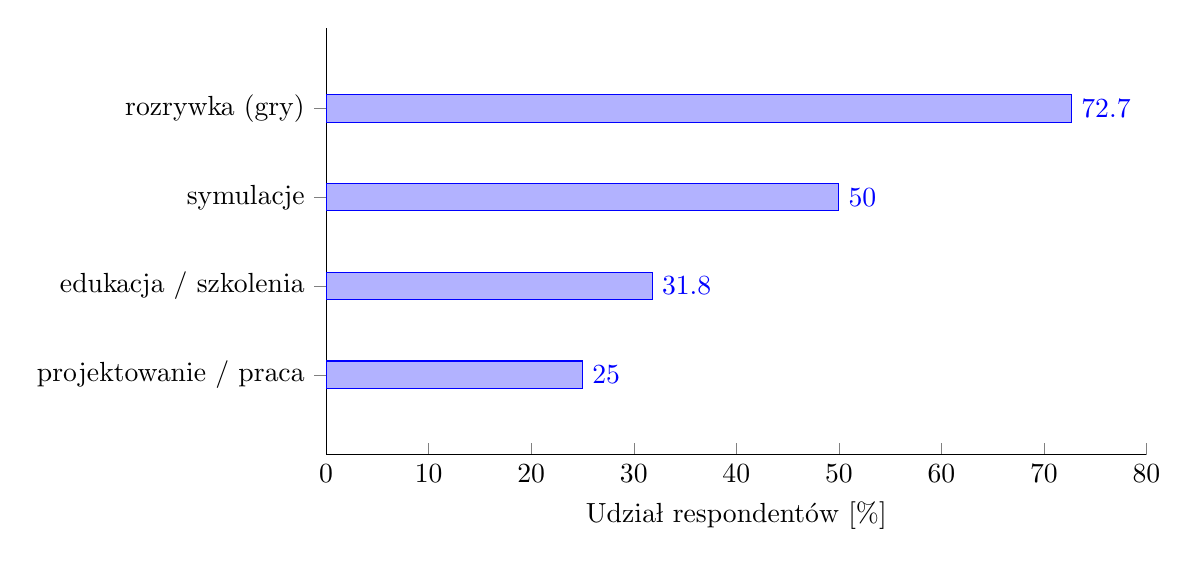
\begin{tikzpicture}
\begin{axis}[
    xbar,
    xmin=0,
    xmax=80,
    width=12cm,
    height=7cm,
    xlabel={Udział respondentów [\%]},
    ytick={1,2,3,4},
    yticklabels={
        rozrywka (gry),
        symulacje,
        edukacja / szkolenia,
        projektowanie / praca
    },
    y dir=reverse,
    nodes near coords,
    nodes near coords align={horizontal},
    bar width=10pt,
    enlarge y limits=0.3,
    axis x line*=bottom,
    axis y line*=left
]
\addplot coordinates {
    (72.7,1)
    (50.0,2)
    (31.8,3)
    (25.0,4)
};
\end{axis}
\end{tikzpicture}
\caption{Cele korzystania z aplikacji i gier VR (wyniki procentowe, możliwość wielokrotnego wyboru, N=44)}
\label{fig:cele_vr_proc}
\end{figure}

\subsection{Poczucie immersji i obecności}

Kolejnym badanym aspektem było poczucie immersji i obecności użytkownika w środowisku wirtualnym oraz wpływ interfejsu i mechanizmów interakcji na ciągłość jego doświadczenia.  Głównym celem tej sekcji było przede wszystkim sprawdzenie, czy interfejs użytkownika w ogóle wpływa na poczucie zanurzenia w VR oraz w jakim stopniu rozwiązania interfejsowe wspierały iluzję obecności, a w jakich sytuacjach prowadziły do jej zaburzenia. Ankietowani mieli odnieść się do swoich wrażeń związanych z poczuciem "zanurzenia" oraz do spójności elementów ze światem wirtualnym. Odpowiedzi pokazują, że interfejs oraz sposób interakcji rzeczywiście wpływają na jakość doświadczenia. Kluczową rolę odgrywała spójność z prezentowanym światem, która najsilniej kształtowała poczucie immersji. Gdy elementy sterowania były odbierane jako sztuczne, niepasujące do kontekstu lub wymagające zbyt dużej koncentracji, ogólne doświadczenie stawało się słabsze. 

\begin{figure}[htbp]
\centering
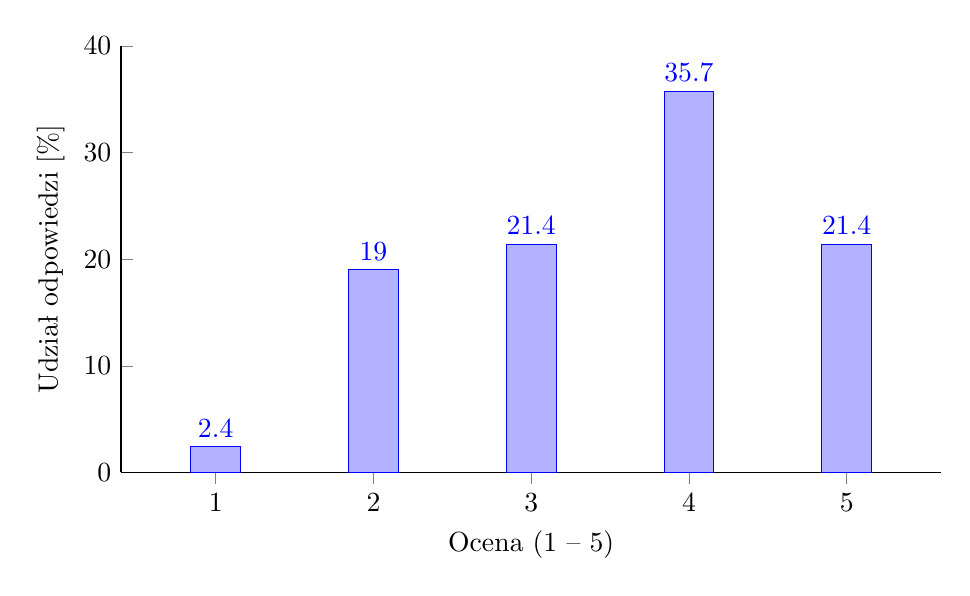
\begin{tikzpicture}
\begin{axis}[
    ybar,
    ymin=0,
    ymax=40,
    width=12cm,
    height=7cm,
    xlabel={Ocena (1 -- 5)},
    ylabel={Udział odpowiedzi [\%]},
    symbolic x coords={1,2,3,4,5},
    xtick=data,
    nodes near coords,
    nodes near coords align={vertical},
    bar width=18pt,
    enlarge x limits=0.15,
    axis x line*=bottom,
    axis y line*=left
]
\addplot coordinates {
    (1,2.4)
    (2,19.0)
    (3,21.4)
    (4,35.7)
    (5,21.4)
};
\end{axis}
\end{tikzpicture}
\caption{Poczucie obecności w wirtualnym środowisku podczas korzystania z VR (wyniki procentowe, N=42)}
\label{fig:presence_vr_proc}
\end{figure}

W odpowiedziach otwartych użytkownicy często zwracali uwagę na momenty "wybijania z doświadczenia", związane m.in. z nagłym pojawianiem się menu, brakiem płynności przejść między interakcjami lub niejednoznacznymi reakcjami systemu. Takie sytuacje mogą być mocno odczuwalne podczas pierwszej styczności z VR, kiedy użytkownik nie ma świadomości, czego się może spodziewać i głównie polega na intuicji oraz wskazówkach od interfejsu. Część respondentów zwróciła również uwagę, że ich zdaniem dobrze zaprojektowane interakcje były spójne z ruchem ciała i otoczeniem. Takie podejście projektowe, według ankietowanych, wzmacniało poczucie obecności i pozwalało na naturalne zanurzenie się w wirtualnym świecie. Najczęściej dotyczyło to rozwiązań, w których interfejs nie narzucał się odbiorcy i nie dominował całego pola widzenia, a informacje były przekazywane w sposób subtelny i tylko wtedy, gdy były rzeczywiście potrzebne. Uzyskane w tej sekcji odpowiedzi potwierdzają, że poczucie immersji w VR jest zależne od jakości interfejsu oraz sposobu realizacji interakcji. Niewielkie niespójności w tym obszarze mogą doprowadzić do zaburzenia doświadczenia i zniechęcić do ponownego korzystania z technologii. 

\begin{figure}[htbp]
\centering
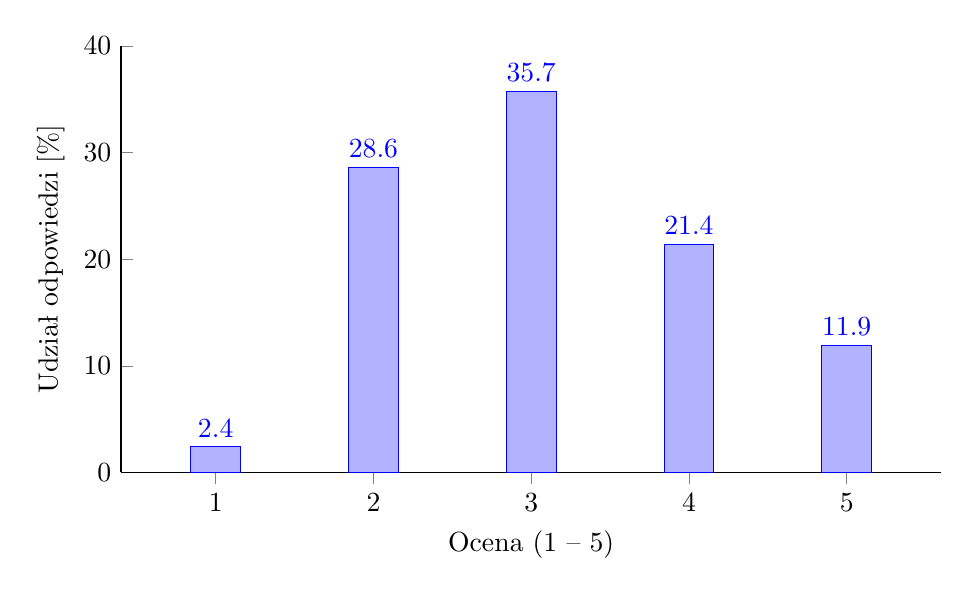
\begin{tikzpicture}
\begin{axis}[
    ybar,
    ymin=0,
    ymax=40,
    width=12cm,
    height=7cm,
    xlabel={Ocena (1 -- 5)},
    ylabel={Udział odpowiedzi [\%]},
    symbolic x coords={1,2,3,4,5},
    xtick=data,
    nodes near coords,
    nodes near coords align={vertical},
    bar width=18pt,
    enlarge x limits=0.15,
    axis x line*=bottom,
    axis y line*=left
]
\addplot coordinates {
    (1,2.4)
    (2,28.6)
    (3,35.7)
    (4,21.4)
    (5,11.9)
};
\end{axis}
\end{tikzpicture}
\caption{Ocena spójności interfejsu i interakcji z otoczeniem wirtualnym (wyniki procentowe)}
\label{fig:ui_spojnosc_vr_proc}
\end{figure}

\subsection{Interakcja i kontrola}

Następny analizowany obszar dotyczył sposobów interakcji z interfejsem, w szczególności celowania, chwytania i przemieszczania się w wirtualnym środowisku. W tej części ankiety respondenci wskazywali na najmniej komfortowe lub mało intuicyjne rozwiązania, jakie napotkali podczas korzystania z symulatorów i gier VR. W odpowiedziach otwartych ankietowani zgłaszali trudności z trafnym wskazaniem niewielkich przycisków laserem oraz dłuższym podtrzymywaniem ręki w tej samej pozycji. Tego typu rozwiązania były przez nich opisywane jako męczące i irytujące. Wyjątkowo nieudanym rozwiązaniem projektowym według nich było menu przypominające te, które spotykają w grach 2D.

Kolejnym często wymienianym problemem było chwytanie i manipulacja obiektami. Jak pisali respondenci, mimo wykonania gestu złapania obiektu, system nie zawsze reagował tak, jak się tego spodziewali. Prowadziło to do frustracji i poczucia utraty kontroli. Trudności dotyczyły również momentu puszczenia obiektu, np podczas rzucania. W kilku odpowiedziach zwracano uwagę, że chwytanie, czyli podstawowa forma kontaktu użytkownika ze środowiskiem wirtualnym, jest nadal zbyt oporna i często zawodzi. 

\begin{figure}[htbp]
\centering
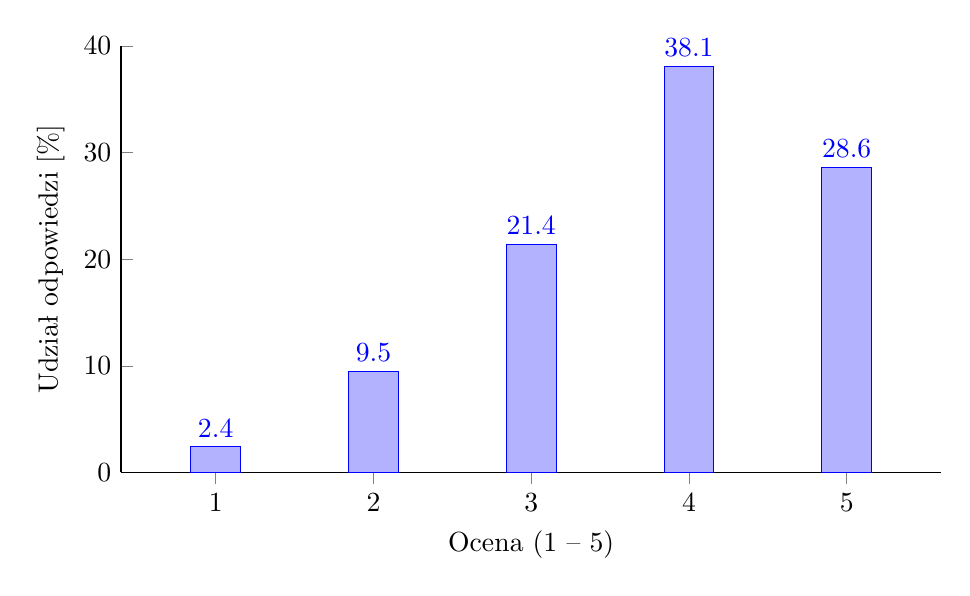
\begin{tikzpicture}
\begin{axis}[
    ybar,
    ymin=0,
    ymax=40,
    width=12cm,
    height=7cm,
    xlabel={Ocena (1 -- 5)},
    ylabel={Udział odpowiedzi [\%]},
    symbolic x coords={1,2,3,4,5},
    xtick=data,
    nodes near coords,
    nodes near coords align={vertical},
    bar width=18pt,
    enlarge x limits=0.15,
    axis x line*=bottom,
    axis y line*=left
]
\addplot coordinates {
    (1,2.4)
    (2,9.5)
    (3,21.4)
    (4,38.1)
    (5,28.6)
};
\end{axis}
\end{tikzpicture}
\caption{Ocena zgodności reakcji systemu z oczekiwaniami użytkownika podczas wykonywania ruchów w VR (wyniki procentowe)}
\label{fig:reakcje_systemu_vr_proc}
\end{figure}

Problematyczne okazało się również przemieszczanie się. Była to najczęściej powtarzająca się odpowiedz w tej sekcji. Część respondentów wskazywało, że płynne poruszanie powodowało u nich mdłości, zawroty głowy lub dyskomfort. Lepszą, lecz nie idealną alternatywą ich zdaniem była teleportacja punktowa. W odpowiedziach otwartych pojawiły się również komentarze sugerujące, że najlepszym rozwiązaniem byłoby poruszanie się wynikające z rzeczywistej pracy ciała.

\begin{figure}[htbp]
\centering
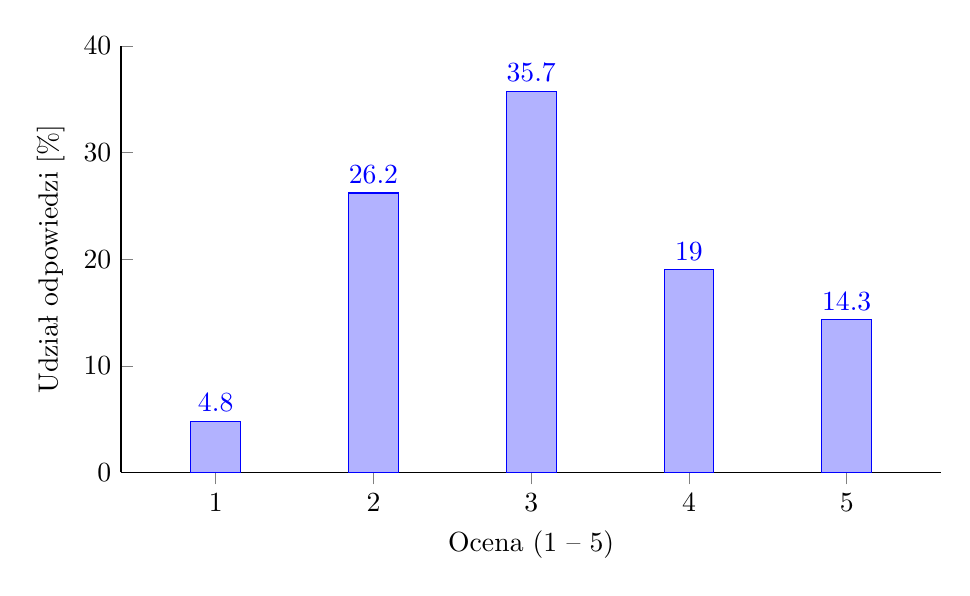
\begin{tikzpicture}
\begin{axis}[
    ybar,
    ymin=0,
    ymax=40,
    width=12cm,
    height=7cm,
    xlabel={Ocena (1 -- 5)},
    ylabel={Udział odpowiedzi [\%]},
    symbolic x coords={1,2,3,4,5},
    xtick=data,
    nodes near coords,
    nodes near coords align={vertical},
    bar width=18pt,
    enlarge x limits=0.15,
    axis x line*=bottom,
    axis y line*=left
]
\addplot coordinates {
    (1,4.8)
    (2,26.2)
    (3,35.7)
    (4,19.0)
    (5,14.3)
};
\end{axis}
\end{tikzpicture}
\caption{Ocena precyzji i łatwości manipulowania elementami interfejsu w środowisku VR (wyniki procentowe)}
\label{fig:manipulacja_interfejs_vr_proc}
\end{figure}

Wszystkie dotychczasowe wypowiedzi użytkowników sugerują, że trudności z interakcją nie wynikają bezpośrednio z zastosowanej technologii, lecz z niespójnego bądź nieprzemyślanego sposobu jej użycia. Te same mechanizmy interakcji mogą w jednej grze funkcjonować bez zarzutu, a w innej prowadzić do irytacji. Jest to szczególnie widoczne wtedy, gdy rozwiązania znane z tradycyjnych gier komputerowych są bezkrytycznie przenoszone do środowiska VR lub gdy ignoruje się kontekst ich realnego wykorzystania w wirtualnej przestrzeni. Zgromadzone odpowiedzi pokazują, że celowanie, chwytanie obiektów oraz poruszanie się należą do najbardziej problematycznych obszarów projektowania interakcji w VR, a ich nieintuicyjne zaprojektowanie może szybko prowadzić do zmęczenia i frustracji. Silnie wpływa to na ogólną ocenę doświadczenia, zwłaszcza podczas pierwszego kontaktu z technologią VR.

\subsection{Komfort i ergonomia}

Kolejna część ankiety dotyczyła ergonomii oraz komfortu korzystania ze środowiska VR. Pytania obejmowały zarówno poziom odczuwanego wysiłku fizycznego, jak i subiektywne dolegliwości, takie jak dezorientacja, trudności z koncentracją czy symptomy choroby lokomocyjnej, bezpośrednio powiązane z przebywaniem w wirtualnym otoczeniu. Zróżnicowane odpowiedzi na pytania zamknięte sugerują, że komfort użytkowania był w dużej mierze uzależniony od zastosowanych rozwiązań interfejsu oraz przyjętych mechanizmów interakcji. Część badanych zgłaszała brak istotnych dolegliwości podczas korzystania z technologii, jednak liczna grupa wskazywała, że szczególnie w trakcie dłuższych sesji pojawiały się takie problemy, jak zmęczenie i dyskomfort oczu czy trudności z utrzymaniem skupienia.

W wypowiedziach otwartych najczęściej pojawiającą się uwagą był konieczność długotrwałego utrzymywania rąk w jednej pozycji w celu wykonania określonej czynności. Respondenci zwracali również uwagę na problemy z czytelnością elementów interfejsu, takie jak niewystarczający kontrast czy zbyt mały rozmiar tekstu. Pojawiały się też komentarze wskazujące, że kluczowe dla rozgrywki elementy były umieszczone poza naturalnym polem widzenia użytkownika. Wszystkie te czynniki prowadziły do szybszego zmęczenia oraz obniżenia subiektywnie postrzeganej jakości rozgrywki.

Uzyskane odpowiedzi wskazują, że komfort i ergonomia mają znaczenie dla odbiorców i stanowią kolejny ważny obszar przy projektowaniu interfejsu oraz mechanizmów interakcji. Rozwiązania wymagające od odbiorcy nadmiernego wysiłku fizycznego lub długotrwałego skupienia uwagi zwiększają ryzyko zmęczenia i dezorientacji, co w konsekwencji może prowadzić do skrócenia czasu korzystania z aplikacji lub rezygnacji z dalszego użytkowania.

\subsection{Informacja zwrotna i opóźnienia}

Ostatnim analizowanym obszarem był czas reakcji systemu oraz sposób przekazywania informacji zwrotnych. Przez informację zwrotną rozumiano wszelkie sygnały wysyłane przez system, które potwierdzają pomyślne wykonanie akcji, zmianę stanu lub pojawienie się błędu. Na podstawie odpowiedzi na pytania zamknięte można stwierdzić, że informacja zwrotna nie stanowiła dla respondentów głównego źródła trudności i była zazwyczaj oceniana pozytywnie. Respondenci rzadko wskazywali ją jako istotny problem. W odpowiedziach na pytania otwarte jako przykład najbardziej udanego rozwiązania najczęściej wskazywano „\textit{Feedback multimodalny}”. Pojawiły się pojedyncze krytyczne uwagi dotyczące informacji zwrotnej, jednak zgłaszane problemy wynikały głównie z niewłaściwego wykorzystania feedbacku w konkretnych realizacjach (np. zastosowanie wyłącznie feedbacku wizualnego), a nie z samej roli informacji zwrotnej w interfejsach VR. W dalszej części ankiety pojawiły się bardziej zróżnicowane opinie dotyczące opóźnień w reakcji systemu i ich wpływu na płynność doświadczenia w VR. Dla części respondentów reakcje systemu były wystarczająco szybkie i nie wpływały istotnie na komfort użytkowania, natomiast inni użytkownicy wskazywali, że nawet niewielkie opóźnienia prowadziły do obniżenia poczucia kontroli i zaburzenia ciągłości doświadczenia.

\begin{figure}[htbp]
\centering
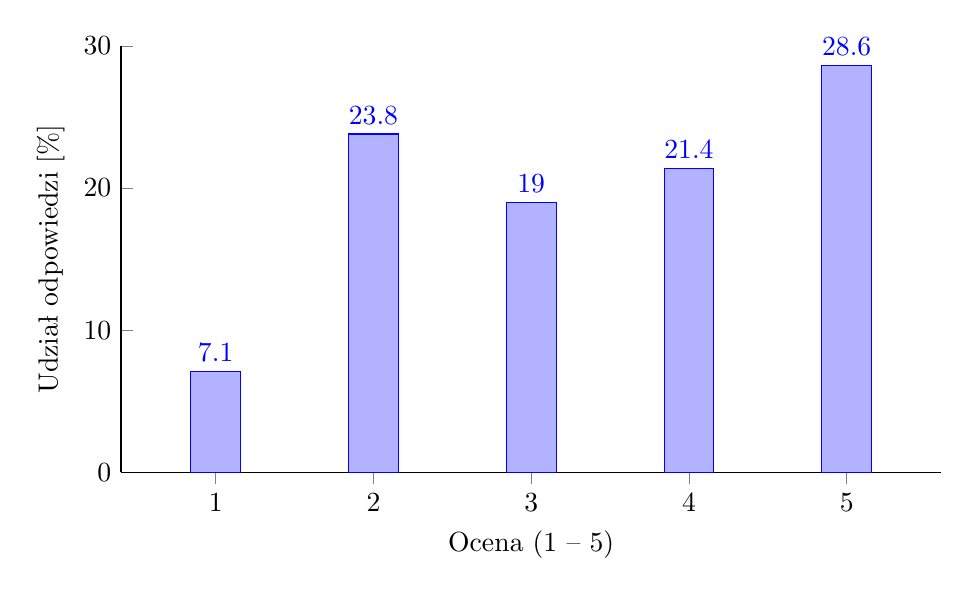
\begin{tikzpicture}
\begin{axis}[
    ybar,
    ymin=0,
    ymax=30,
    width=12cm,
    height=7cm,
    xlabel={Ocena (1 -- 5)},
    ylabel={Udział odpowiedzi [\%]},
    symbolic x coords={1,2,3,4,5},
    xtick=data,
    nodes near coords,
    nodes near coords align={vertical},
    bar width=18pt,
    enlarge x limits=0.15,
    axis x line*=bottom,
    axis y line*=left
]
\addplot coordinates {
    (1,7.1)
    (2,23.8)
    (3,19.0)
    (4,21.4)
    (5,28.6)
};
\end{axis}
\end{tikzpicture}
\caption{Ocena wpływu opóźnień w reakcji interfejsu na doświadczenie użytkownika w VR (wyniki procentowe)}
\label{fig:opoznienia_interfejs_vr_proc}
\end{figure}

Zróżnicowanie tych ocen można wyjaśniać indywidualnymi różnicami w postrzeganiu upływu czasu oraz wcześniejszymi doświadczeniami użytkowników z technologią VR i grami cyfrowymi. Jak podkreśla Jason Jerald w książce „\textit{The VR Book}”, próg wykrywania opóźnień nie jest wartością stałą i zależy między innymi od stopnia obycia użytkownika z systemami interaktywnymi oraz od sposobu integracji bodźców wzrokowo-ruchowych. W praktyce oznacza to, że identyczny poziom opóźnienia może dla jednych użytkowników mieścić się w granicach akceptowalności, podczas gdy dla innych będzie już przekraczał próg detekcji, co skutkuje spadkiem poczucia immersji i kontroli. Wyniki tej części ankiety sugerują, że mimo iż informacja zwrotna w analizowanych doświadczeniach była przeważnie oceniana pozytywnie, to redukcja opóźnień systemu wciąż stanowi kluczowy warunek wysokiej jakości interakcji w VR. Nawet relatywnie niewielkie opóźnienia, połączone z brakiem jednoznacznej reakcji systemu, mogą wywoływać frustrację i prowadzić do negatywnej oceny całego doświadczenia.

\section{Wnioski i odniesienie do pytań badawczych}

Przeprowadzone badania wstępne pozwoliły na jakościową identyfikację kluczowych problemów związanych z projektowaniem interfejsów użytkownika oraz mechanizmów interakcji w grach VR. Otrzymane wyniki potwierdzają, że doświadczenia użytkownika w środowisku wirtualnym nie wynikały wyłącznie z samego wyboru technik, lecz sposobu ich implementacji, spójności z kontekstem użycia i przewidywalności reakcji systemu. Jednym z najistotniejszych wniosków jest silny związek pomiędzy jakością interfejsu a poczuciem immersji i obecności.

\subsection{Wnioski}

Elementy interfejsu, które zbyt mocno narzucają się użytkownikowi i pochłaniają nadmierną uwagę, są postrzegane przez odbiorców jako niezgodne z logiką świata wirtualnego, co prowadzi do przerwania ciągłości doświadczenia. Rozwiązania zakorzenione w kontekście świata gry, subtelne i ściśle powiązane z działaniami użytkownika, sprzyjają utrzymaniu nieprzerwanego zanurzenia w środowisku wirtualnym. Analiza odpowiedzi dotyczących interakcji ujawniła, że celowanie, chwytanie oraz poruszanie się stanowią najbardziej newralgiczne obszary projektowe. Problemy zgłaszane przez użytkowników nie dotyczyły pojedynczych technik jako takich, lecz ich niespójnej realizacji, niskiej precyzji lub bezrefleksyjnego przenoszenia rozwiązań znanych z gier komputerowych do środowiska VR. Szczególnie widoczne było to w przypadku płaskich menu, obsługiwanych najczęściej niewygodnym według ankietowanych wskaźnikiem laserowym. Problematyczna była również zawodność mechanizmów chwytania, która prowadziła do frustracji i poczucia utraty kontroli.

W obszarze komfortu badania wykazały że rozwiązania wymagające długotrwałego utrzymywania rąk w jednej pozycji, wysokiej precyzji gestów lub stałego skupienia wzroku na drobnych elementach interfejsu istotnie obniżają jakość doświadczenia. Problemy te były szczególnie dotkliwe podczas dłuższych sesji i mogły prowadzić do zmęczenia, dezorientacji oraz skrócenia czasu korzystania z aplikacji. Zróżnicowanie ocen dotyczących opóźnień reakcji systemu wskazuje, że jest to czynnikiem silnie zależnym od indywidualnych cech użytkowników oraz ich wcześniejszego doświadczenia z technologią VR. Te same opóźnienia mogą być przez jednych odbierane jako akceptowalne lub niezauważalne, podczas gdy u innych prowadzą do wyraźnego obniżenia poczucia kontroli i płynności doświadczenia. Potwierdza to, że czas reakcji systemu jest istotnym elementem wpływającym na jakość interakcji w środowiskach VR. Zebrane wyniki stanowią podstawę do sformułowania założeń projektowych dla dalszego etapu pracy, obejmującego projektowanie i implementację prototypów gry VR. Wskazują na konieczność projektowania interfejsu w sposób kontekstowy, ergonomiczny i spójny z logiką świata wirtualnego, z naciskiem na przewidywalność reakcji systemu, minimalizowanie opóźnień oraz ograniczenie rozwiązań wymagających nadmiernego wysiłku fizycznego lub poznawczego.

\subsection{Odniesienie do pytań badawczych}

Na podstawie wyników ankiety można sformułować następujące odpowiedzi na pytania badawcze:

\begin{enumerate}
    \item Najbardziej zakłócające immersję i poczucie obecności były elementy interfejsu narzucające się użytkownikowi oraz rozwiązania postrzegane jako oderwane od logiki świata wirtualnego. Respondenci wskazywali m.in. na nagłe pojawianie się menu, brak płynności przejść między interakcjami oraz niejednoznaczne reakcje systemu, które „wybijały” z doświadczenia.
    \item Intuicyjność i precyzja interakcji wpływały na doświadczenie, szczególnie w obszarze podstawowych czynności: celowania, chwytania i nawigacji. Za mało intuicyjne uznawano między innymi manipulowanie drobnymi elementami wskaźnikiem laserowym oraz rozwiązania przeniesione z gier 2D.
    \item Dyskomfort fizyczny i percepcyjny wiązał się przede wszystkim z lokomocją (mdłości i zawroty głowy przy płynnym poruszaniu się). Respondenci wskazywali na zmęczenie wynikające z długotrwałego utrzymywania rąk w jednej pozycji, a także na problemy z czytelnością (zbyt mały tekst, niewłaściwy kontrast) oraz na elementy umieszczone poza naturalnym polem widzenia.
    \item Brak lub opóźnienie informacji zwrotnej rzadko stanowiły główny problem, jednak opóźnienia reakcji systemu były oceniane bardziej zróżnicowanie i u części użytkowników obniżały poczucie kontroli oraz płynność doświadczenia. Najlepiej oceniano informację zwrotną wielomodalną, a negatywne oceny dotyczyły głównie sytuacji, w których feedback był niejednoznaczny lub ograniczony do jednego kanału (np. wyłącznie wizualnego).
\end{enumerate}